%FOR PDFLATEX USE ONLY
\documentclass[a4paper,12pt]{article}

\usepackage{amssymb,amsmath}

\usepackage[margin=2cm]{geometry}
\usepackage[unicode]{hyperref}
\usepackage[pdftex]{graphicx}
\usepackage{cmlgc}

\usepackage{array}

\usepackage{wrapfig}
\usepackage{array}
\usepackage{lipsum}
\usepackage{esvect}
\usepackage{hyperref}

\usepackage{subfig}
\usepackage{calc}
\usepackage{pgfplots,tikz,circuitikz}
\usepackage{pgfplotstable}
\usepackage{tkz-euclide}

\usepackage{centernot}
\usepackage{cancel}

\usepackage{mathtext}
\usepackage[T1,T2a]{fontenc}
\usepackage[utf8]{inputenc}
\usepackage[english, bulgarian, russian]{babel}
\usepackage{tikz}
\usepackage{pgfplots}
\usepackage[export]{adjustbox}
\usepackage[left=2cm,right=2cm,
    top=2cm,bottom=2cm,bindingoffset=0cm]{geometry}
\usepackage{indentfirst}
\usepackage{braket}
\include{data_40_1}

\begin{document}

\begin{center}
  \LARGE{Лабораторная работа -- вопрос по выбору}\\[0.2cm]
  \LARGE{Жидкостный и газовый термометр}\\[0.2cm]
  \large{Панферов Андрей}\\[0.2cm]
\end{center}  
  
\section{Аннотация}
В работе собирается 2 термометра: жидкостный и газовый, а так же исследуется их работоспособность и границы применимости для разных условий. 

\section{Теоретические сведения}
\textit{Газовый термометр} — прибор для измерения температуры, основанный на законе Шарля.



\textbf{Принцип работы}\\

В конце XVIII в. Шарль установил, что одинаковое нагревание любого газа приводит к одинаковому повышению давления, если при этом объём остается постоянным. При изменении температуры по шкале Цельсия зависимость давления газа при постоянном объёме выражается линейным законом. А отсюда следует, что давление газа при постоянном можно принять в качестве количественной меры температуры. Соединив сосуд, в котором находится газ, с манометром и проградуировав прибор, можно измерять температуру по показаниям манометра.

В широких пределах изменений концентраций газов и температур и малых давлениях температурный коэффициент давления разных газов примерно одинаковый, поэтому способ измерения температуры с помощью газового термометра оказывается малозависящим от свойств конкретного вещества, используемого в термометре в качестве рабочего тела. Наиболее точные результаты получаются, если в качестве рабочего тела использовать водород или гелий.

\textbf{Примеры:}\\

\begin{minipage}{0.45\textwidth} 
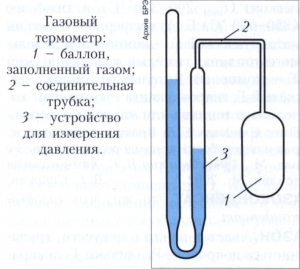
\includegraphics[width=\linewidth]{1.png}\\
\end{minipage}
\begin{minipage}{0.07\textwidth}
\
\end{minipage}
\begin{minipage}{0.45\textwidth}
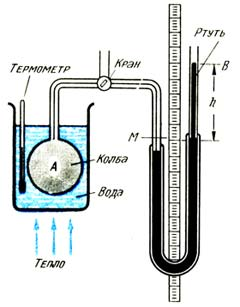
\includegraphics[width=0.7\linewidth]{2.jpg}\\
\end{minipage}
\newpage
\textit{Жи́дкостный термо́метр} -- прибор для измерения температуры, действие которого основано на термическом расширении жидкости.\\

\begin{minipage}{0.45\textwidth} 
Принцип действия стеклянных жидкостных термометров основан на тепловом расширении термометрической жидкости, заключенной в термометре. При этом, очевидно, показания жидкостного термометра зависят не только от изменения объема термометрической жидкости, но также и от изменения объема стеклянного резервуара, в котором находится эта жидкость. Таким образом, наблюдаемое (видимое) изменение объема жидкости преуменьшено на размер, соответственно равный увеличению объема резервуара (и частично капилляра). Для заполнения жидкостных термометров применяют ртуть, толуол, этиловый спирт, керосин, петролейный эфир, пентан и т. д.\\
\end{minipage}
\begin{minipage}{0.07\textwidth}
\
\end{minipage}
\begin{minipage}{0.45\textwidth}
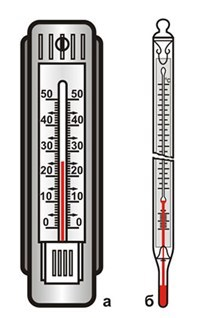
\includegraphics[width=0.7\linewidth]{3.jpeg}\\
\end{minipage}

\section{Оборудование}

\textbf{В работе используются:} шприц на 20 мл, спирт технический, краситель, 2 длинные трубочки (из под моющих средств или компрессоров для аквариума), горячая (закипающая) вода, холодная (замерзающая) вода, пустая баночка из-под антисептика, пустая баночка из-под лекарства, линейка, фломастер, пластилин.  \\

\begin{center}
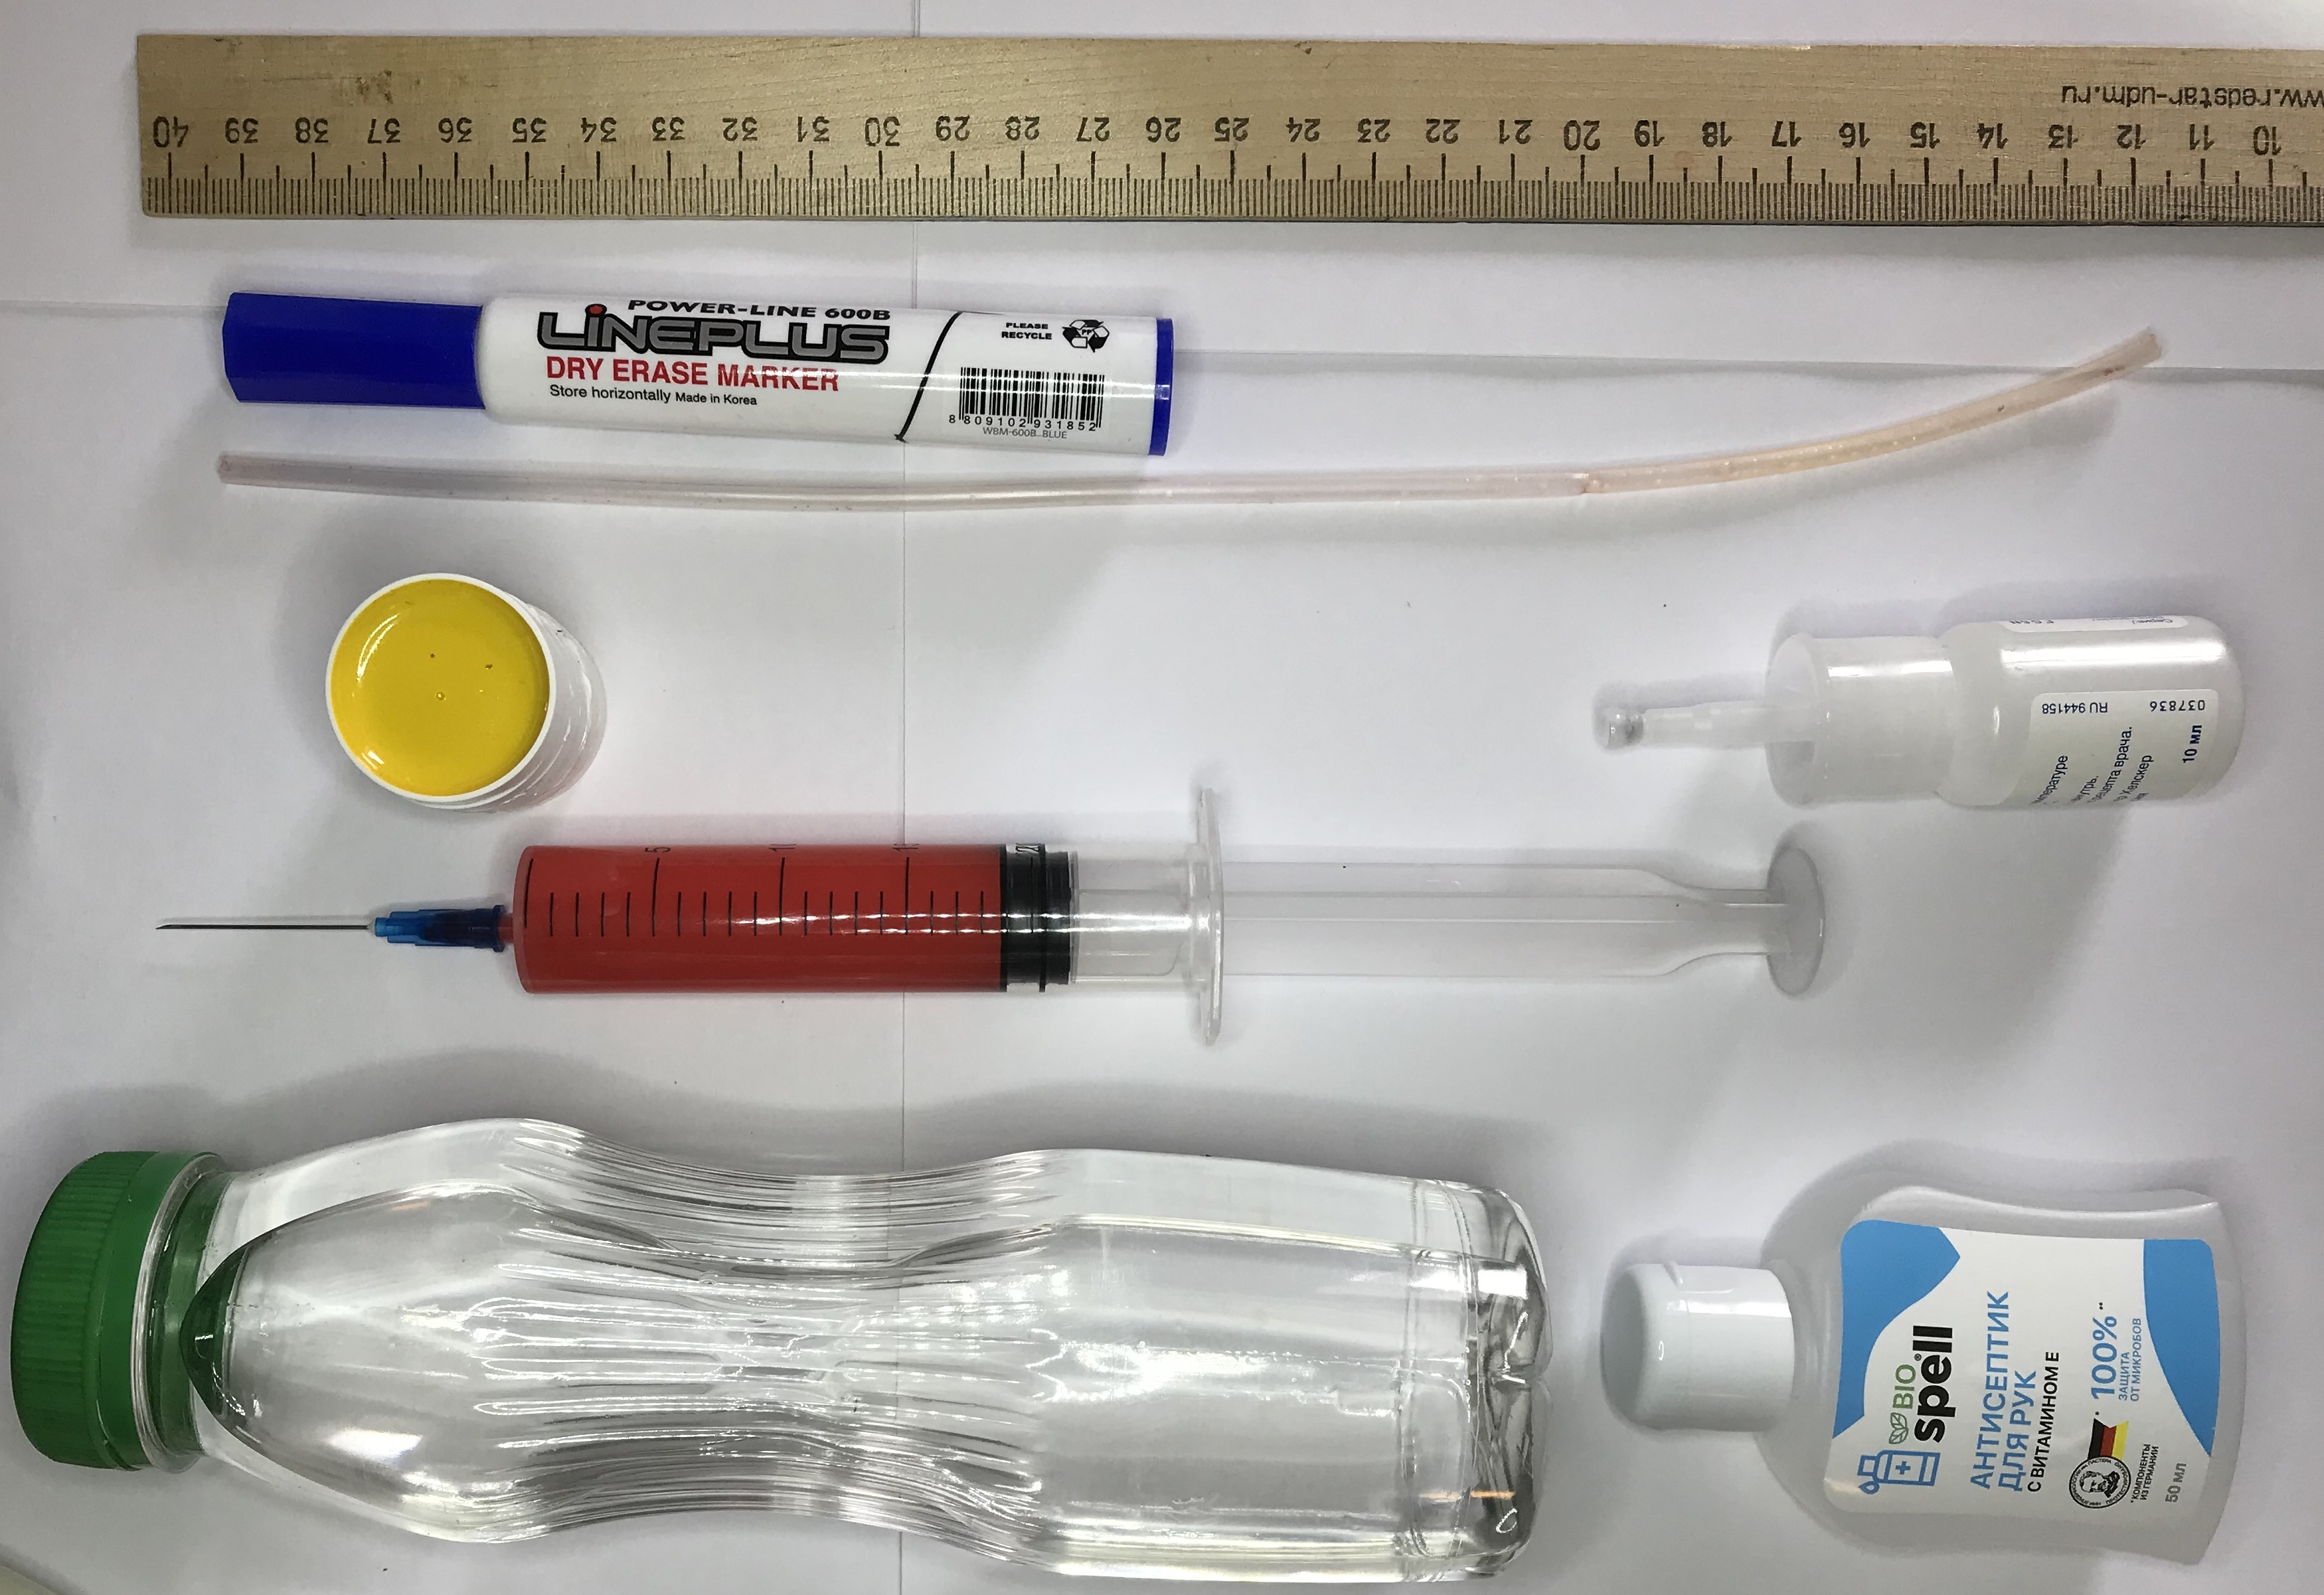
\includegraphics[width=0.9
\linewidth]{4.jpg}\\
\end{center}


\section{Сборка и калибровка термометров}

\subsection{Газовый термометр}

\begin{minipage}{0.3\textwidth}
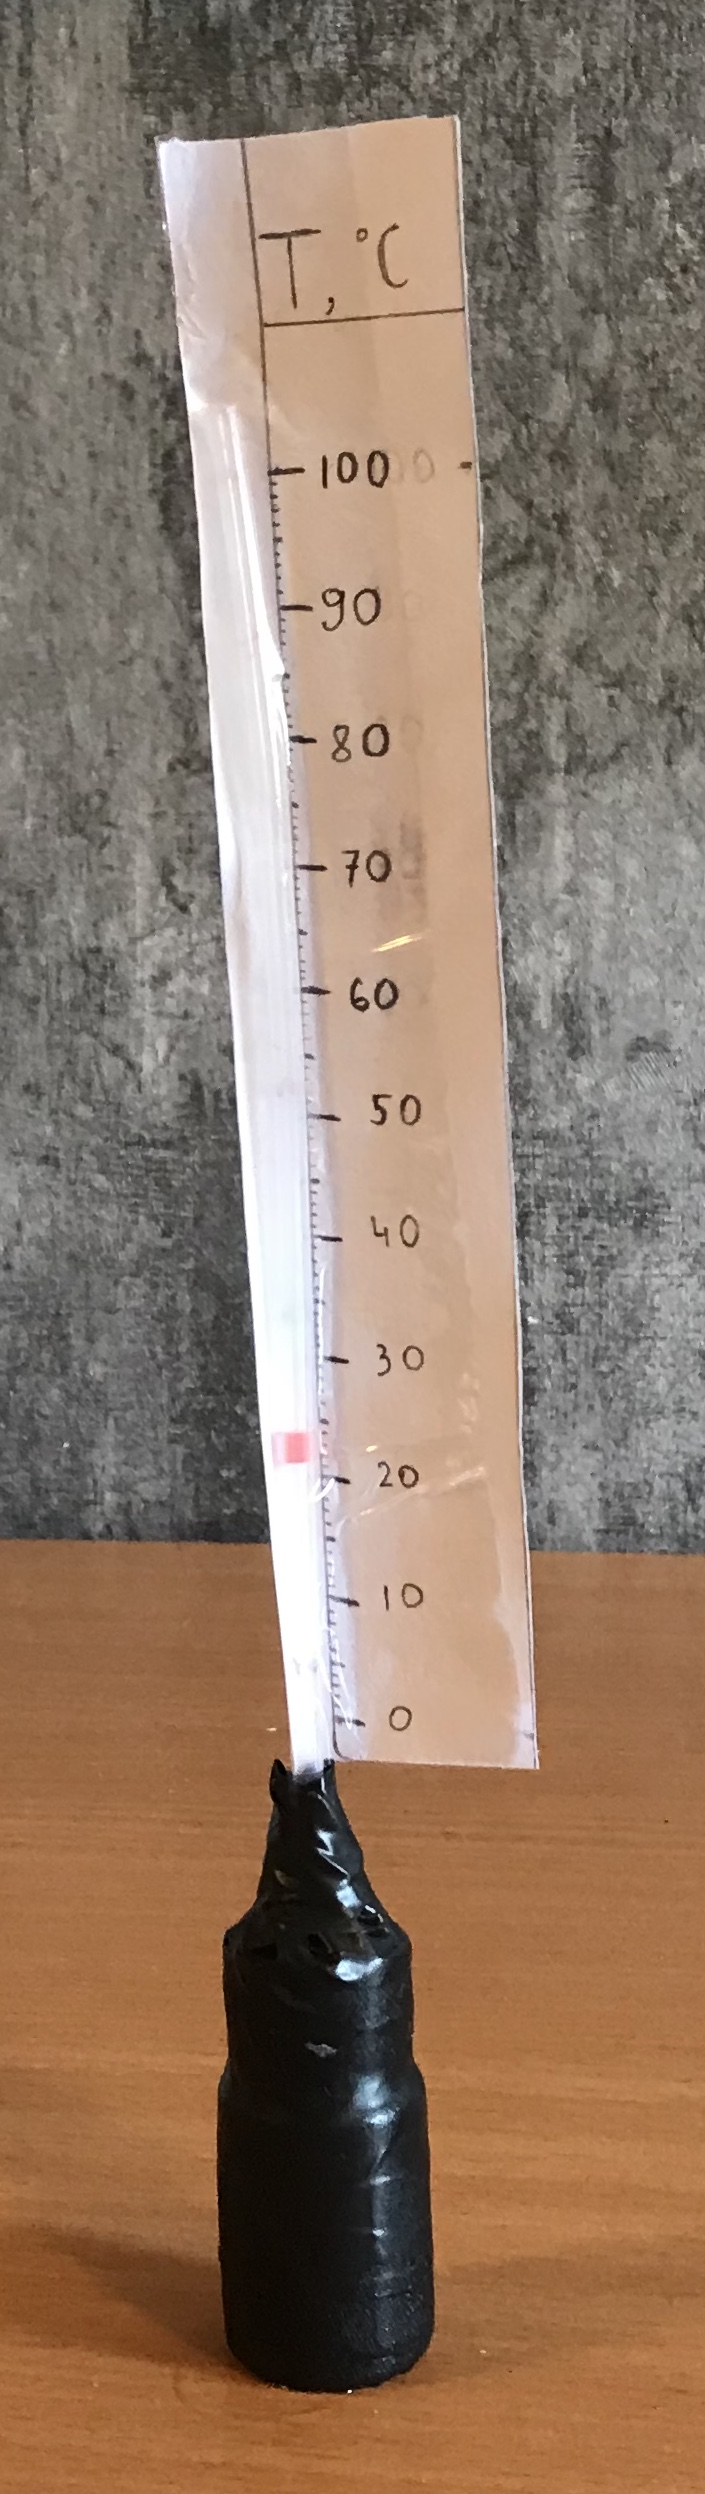
\includegraphics[width=0.9\linewidth]{5.jpg}\\
\end{minipage}
\begin{minipage}{0.07\textwidth}
\
\end{minipage}
\begin{minipage}{0.6\textwidth} 
Из уравнения состояния идеального газа: \[PV = \nu RT \ \ \ \ \ \  P(V+\Delta V) = \nu R(T+\Delta T)\]

Можно сделать вывод, что обьём трубки должен составлять примерно треть обьема баллона для диапазона температур от 273 К до 373 К. \\
Диаметр трубки составляет $d \approx 3$ мм, а её длина, учитывая, что ее часть должна быть внутри сосуда -- составляет примерно 25 см, значит обьем воздуха в сосуде должен составлять 3 - 4 мл. \\

Вставим трубку в сосуд и добавим в неё цветную $"водяную\ пробку"$, чтобы можно было отслеживать координату. 

Окончательно отметим показания при помещении $"устройства"$ в холодную (смесь воды со льдом) и горячую (кипящцю) воду, и так как шкала будет линейной, нанесем окончательную разметку. 

В действительности $"термометр"$ выглядит,  как показано на картинке слева. 
\end{minipage}

\newpage

\subsection{Жидкостный термометр}

\begin{minipage}{0.6\textwidth} 
Согласно табличным данным, температурный коэффициент расширения спирта изменяется не сильно в диапазоне от 0 до 100 градусов Цельсия, и равен $\beta = \frac{1}{V}(\frac{\partial V}{\partial T})_P \approx 1\cdot 10^{-3} K^{-1}$, значит шкала будет тоже линейна, а для того, чтобы температуру измерять было удобно, потребуется примерно 60 мл. \\

Смешаем краситель со спиртом, чтобы было удобнее замечать уровень жидкости. \\

 \ 
 
Аналогично предыдущему пункту соберем и отнормируем термометр. \\

Стоит отметить, чтобы такого рода термометр прослужил дольше, нужно добавить каплю масла поверх слоя жидкости, чтобы последняя н испарялась. \\

Так же стоит отметить, что наличие маленьких пузырьков воздуха внутри такого термометра не будет влиять на его показания в силу линейности изобарического расширения газа. С учетом того, что сосуд герметичен, а так же нормировка проходила после его плотного закрытия, можно убедиться в том, что термометр работает нормально, однако, из-за большого количества жидкости, температурное равновесие между термометром и измеряемым телом происходит достаточно медленно. 

\end{minipage}
\begin{minipage}{0.07\textwidth}
\
\end{minipage}
\begin{minipage}{0.3\textwidth}
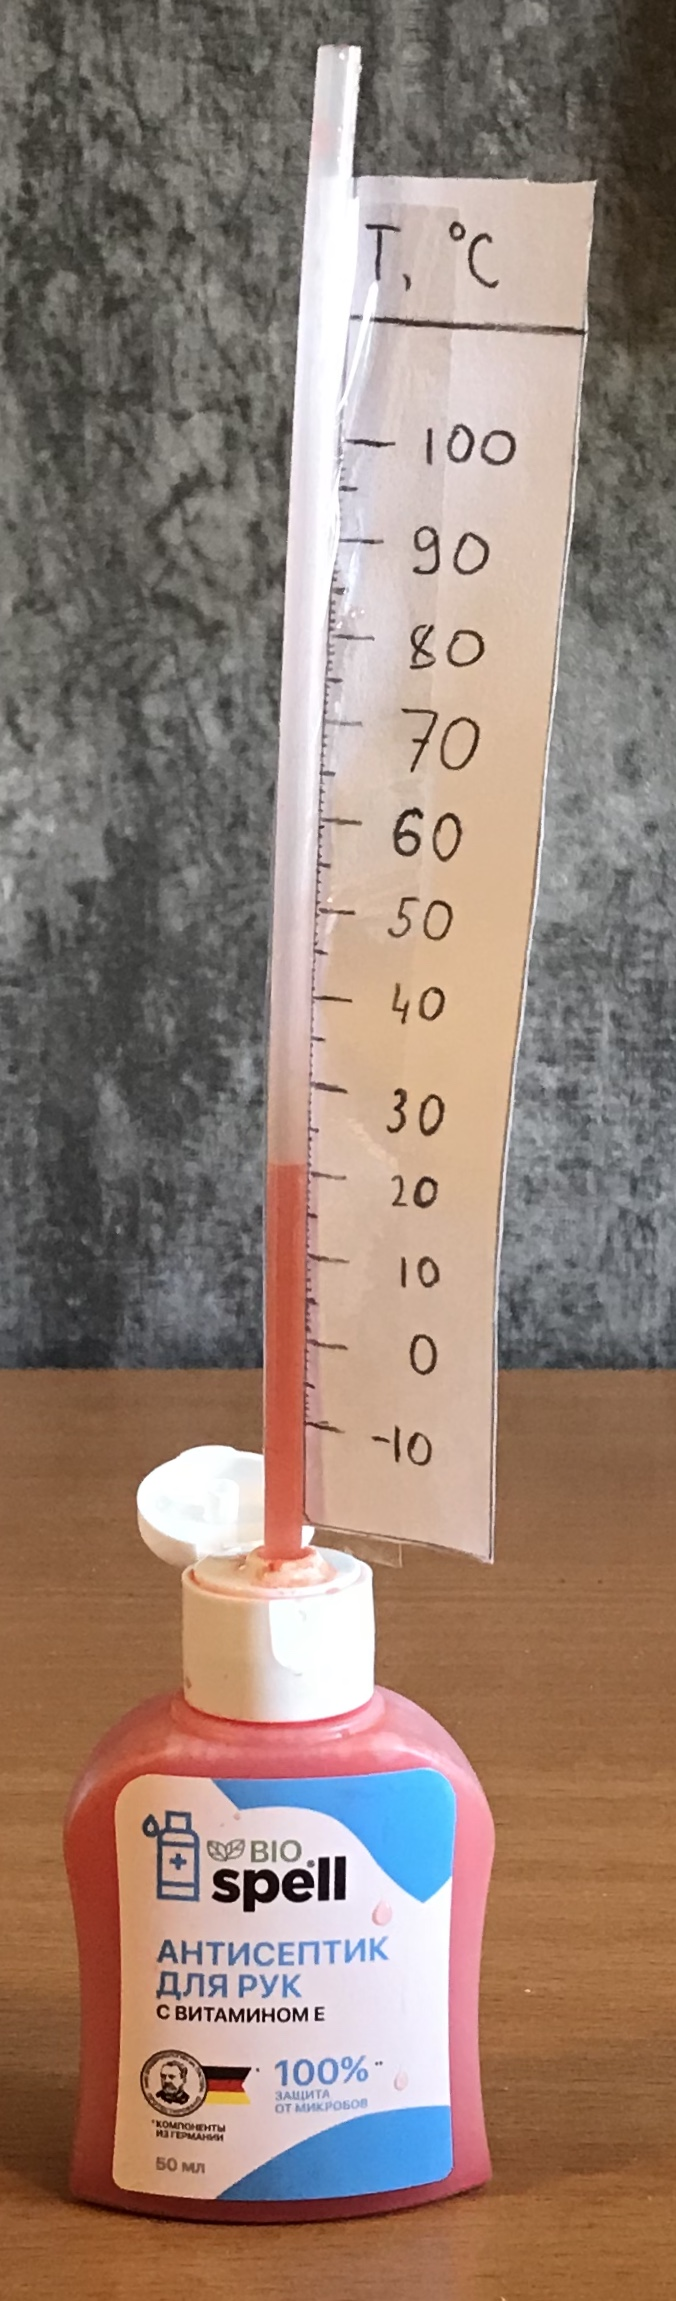
\includegraphics[width=1.2\linewidth]{6.jpg}\\
\end{minipage}

\newpage

\section{Измерения}

\subsection{Комнатная температура}

Как можно видеть на фотографиях устройства, комнатная температура по ним может быть оценена как $\approx 22 \pm 2 C$, при комнатной температуре равной $23C$ (измеренной термометром).

\subsection{Остывание жидкости}

С использованием нашего газового термометра (выбор обоснован большей скоростью отклика показаний на изменения температуры) измерим зависимость температуры воды в кастрюле при ее остывании.\\

Из теории известно, что зависимость должна иметь вид:
\[T(t) = T_0 + (T(t = 0) - T_0)\cdot e^{-\alpha t}\]
, где $T_0$ - температура окружающей среды, $\alpha$ - коэффициент, обоснованный пропорциональностью потерь тепла разности температур с окружающей средой.

Предварительно измерим температуру окружающей среды $T_0 = 22C$.

\begin{table}[h!]
\begin{minipage}{0.2\textwidth}
\begin{tabular}{|l|l|}
\hline
t, мин & T, C \\ \hline
0      & 100  \\ \hline
10     & 75   \\ \hline
20     & 56   \\ \hline
30     & 46   \\ \hline
40     & 39   \\ \hline
50     & 33   \\ \hline
60     & 30   \\ \hline
\end{tabular}
\end{minipage}
\begin{minipage}{0.4\textwidth}
\begin{tikzpicture}[scale=0.8]
	\begin{axis}[
		axis lines = left,
    	xlabel = {t, мин},
    	ylabel = {T, C},
    	ylabel style={black, scale=0.7},
    	xlabel style={black, scale=0.7},
    	ymin=0, ymax=100,
    	title={Зависимость $T$ от $t$},
    	legend style={at={(0.03,-0.4)},anchor=west}
		]
		\addplot+[blue, only marks]  plot[
			error bars/.cd,
			y dir=both,
			y fixed = 2,
		]
		coordinates
		{(0, 100) (10, 75) (20, 51) (30, 46) (40, 39) (50, 33) (60, 30)};
		\addplot[color=black, domain=0:60]{22};
	\end{axis}
\end{tikzpicture}
\end{minipage}
\begin{minipage}{0.35\textwidth}
\begin{tikzpicture}[scale=0.8]
	\begin{axis}[
		axis lines = left,
    	xlabel = {t, мин},
    	ylabel = {$ln(\frac{T - T_0}{T(0) - T_0})$},
    	ylabel style={black, scale=0.7},
    	xlabel style={black, scale=0.7},
    	%ymin=0, ymax=100,
    	title={Зависимость $ln(\frac{T - T_0}{T(0) - T_0})$ от $t$},
    	legend style={at={(0.03,-0.4)},anchor=west}
		]
		\addplot+[blue, only marks]  plot[
			error bars/.cd,
			y dir=both,
			y fixed = 0.13,
		]
		coordinates
		{(0, 0) (10, -0.38) (20, -0.98) (30, -1.17) (40, -1.52) (50, -1.95) (60, -2.27)};
		\addplot[color=red, domain=0:60]{-0.038 * x - 0.02};
	\end{axis}
\end{tikzpicture}
\end{minipage}
\end{table}

Мы видим, что зависимость соответствует предсказаной, что означает, что линейная градуировка термометра - првильный подход.



 \section{Выводы и рассчёт погрешностей}
 \subsection{Погрешности}
Основной вклад в погрешности таких термометров вносят несколько факторов. \\
Во первых, температура кипения воды в реальных условиях немного меньше 100 градусов, в силу того, что давление отличается от табличного, а так же, в воде достаточно много разных примесей в виде солей, минералов. \\
Во вторых, по аналогичным причинам, температура замерзания воды немного ниже 0. \\
В третьих, имеется инструментальная погрешность линейки, которая вносит примерно 1\% вклад в ошибку показаний термометра. \\
В четвертых, отдельно для газового термометра флуктуации в среде вносят значительный вклад в ошибку, так как жидкостная $"пробка"$ немного колеблется вокруг положения равноевсия. \\
Суммируя всё вышесказанное, можно сделать заключение о том, что ошибка газового термометра -- примерно 3 К, а ошибка жидкостного -- примерно 2 К. 
 \subsection{Вывод}
 
 В работе были удачно собраны 2 термометра и сравнены их характеристики. \\
 Каждый термометр имеет свои преимущества и недостатки.\\
 Теоретически, газовый термометр более подходит для измерения большего диапазона температур, так как воздух конденсируется ниже чем 200 К, а ионизируется выше чем 1000 К, однако всё зависит от сосуда, и вещества, используемого в качестве $"пробки"$, так же такой термометр быстрее реагирует на изменения окружающей среды, так как теплоемкость воздуха сильно меньше теплоемкости жидкостей, однако это вносит большую погрешность. \\
 Жидкостный термометр, в теории, имеет меньший диапазон рабочих температур, однако он более точен. \\
 В целом, 2 собранных термометра работают в одних и тех же диапазонах температур так как трубки короткие, однако верхний предел жидкостного может быть достигнут на отметке немногим выше максимальной. \\
 Из минусов можно выделить то, что они достаточно велики для каких-либо лабораторных измерений, а так же то, что их надо держать в строго вертикальном положении, иначе жидкость будет вытекать. При расчете на долгое использование, каждое устройство нужно будет нормировать заново, чтобы быть уверенным в том, что всё работает верно, но в крайнем случае, обе модели вполне работоспособны. 
  


 \end{document}
